\subsection{Integration Testing}
As mentioned briefly earlier, integration testing is the testing of the interaction between classes. After unit testing, we want to gradually piece together our code and the classes interactions with each other, such that for each new interaction we test that it performs as expected. We keep doing this until we have tested all the connections, such that there will not be any unforeseen problems when we put the entire solution together \cite{TestingBlackbox}. \\
There are two ways to go about integration testing: bottom-up and top-down approach. We will look at the bottom-up approach, as this is the approach that we took. 
\subsubsection{Bottom-up Approach}
In the bottom-up approach we start by testing our individual classes, where they are coupled as they would be in the full system, but where we keep them seperated by means of mocking the dependencies. Then, we couple two classes together and perform integration testing on those. After testing the connections between these two classes, we can then continue to add classes to the integration tests one by one, such that we gradually test all the connections of the code \cite{TestingBlackbox}. If we look at \autoref{integrationDia} we can see how we did this. We start by making integration tests of the room and monster, then add player and test this connection to the room and monster. We continue this way until all our connections have been tested. \todo{Perhaps add whole chain?}
\begin{figure}
    \centering
    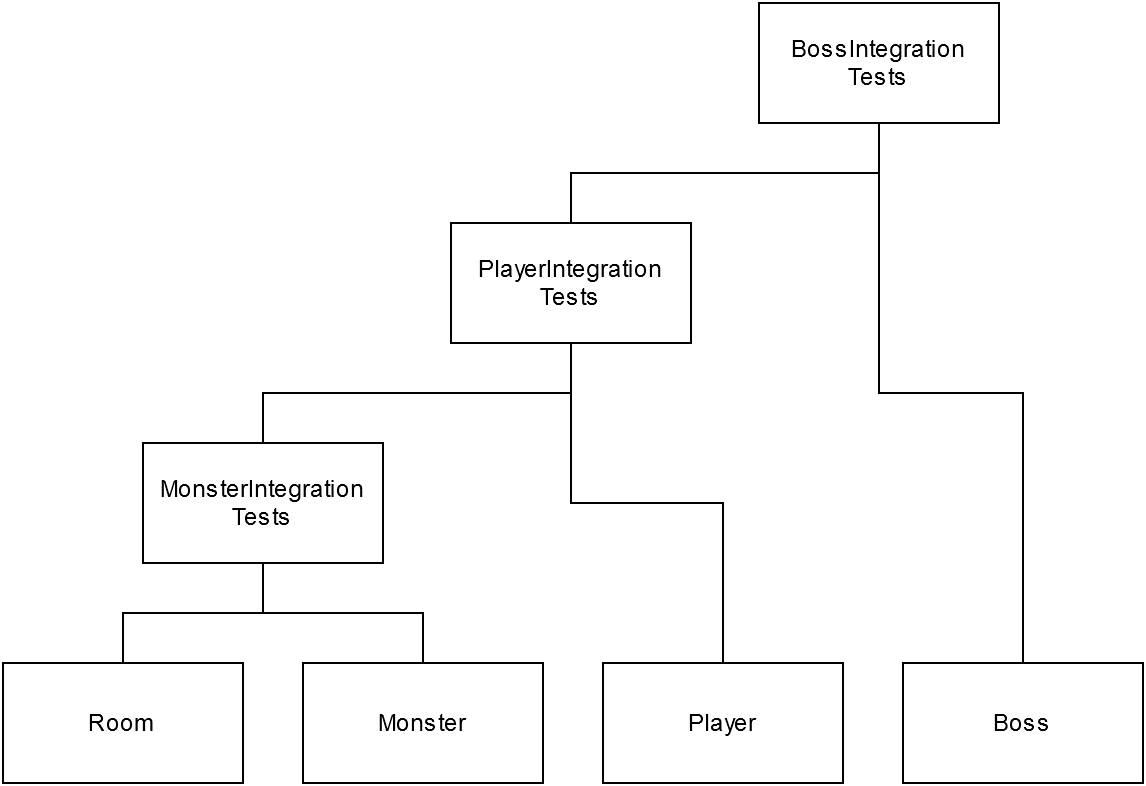
\includegraphics[width=0.7\linewidth]{Materials/TestingTheory/IntegrationDiagram}
    \caption{A diagram showing our means of integration testing.}
    \label{integrationDia}
\end{figure}
